\documentclass[a4paper]{article}
\usepackage{a4wide,amssymb,epsfig,latexsym,multicol,array,hhline,fancyhdr}
\usepackage{vntex}
\usepackage{amsmath}
\usepackage{lastpage}
\usepackage[lined,boxed,commentsnumbered]{algorithm2e}
\usepackage{enumerate}
\usepackage{color}
\usepackage{graphicx}							% Standard graphics package
\usepackage{array}
\usepackage{tabularx, caption}
\usepackage{multirow}
\usepackage{multicol}
\usepackage{rotating}
\usepackage{graphics}
\usepackage{geometry}
\usepackage{setspace}
\usepackage{epsfig}
\usepackage{tikz}
\usetikzlibrary{arrows,snakes,backgrounds}
\usepackage{hyperref}
\hypersetup{urlcolor=blue,linkcolor=black,citecolor=black,colorlinks=true} 
%\usepackage{pstcol} 								% PSTricks with the standard color package

\newtheorem{theorem}{{\bf Theorem}}
\newtheorem{property}{{\bf Property}}
\newtheorem{proposition}{{\bf Proposition}}
\newtheorem{corollary}[proposition]{{\bf Corollary}}
\newtheorem{lemma}[proposition]{{\bf Lemma}}

\AtBeginDocument{\renewcommand*\contentsname{Contents}}
\AtBeginDocument{\renewcommand*\refname{References}}
%\usepackage{fancyhdr}
\setlength{\headheight}{40pt}
\pagestyle{fancy}
\fancyhead{} % clear all header fields
\fancyhead[L]{
 \begin{tabular}{rl}
    \begin{picture}(25,15)(0,0)
    \put(0,-8){
\includegraphics[width=8mm, height=8mm]{hcmut.png}}
    %\put(0,-8){\epsfig{width=10mm,figure=hcmut.eps}}
   \end{picture}&
	%
\includegraphics[width=8mm, height=8mm]{hcmut.png} & %
	\begin{tabular}{l}
		\textbf{\bf \ttfamily University of Technology, Ho Chi Minh City}\\
		\textbf{\bf \ttfamily Faculty of Computer Science and Engineering}
	\end{tabular} 	
 \end{tabular}
}
\fancyhead[R]{
	\begin{tabular}{l}
		\tiny \bf \\
		\tiny \bf 
	\end{tabular}  }
\fancyfoot{} % clear all footer fields
\fancyfoot[L]{\scriptsize \ttfamily Assignment 1 for Database Systems - Academic year 2021 - 2022}
\fancyfoot[R]{\scriptsize \ttfamily Page {\thepage}/\pageref{LastPage}}
\renewcommand{\headrulewidth}{0.3pt}
\renewcommand{\footrulewidth}{0.3pt}


%%%
\setcounter{secnumdepth}{4}
\setcounter{tocdepth}{3}
\makeatletter
\newcounter {subsubsubsection}[subsubsection]
\renewcommand\thesubsubsubsection{\thesubsubsection .\@alph\c@subsubsubsection}
\newcommand\subsubsubsection{\@startsection{subsubsubsection}{4}{\z@}%
                                     {-3.25ex\@plus -1ex \@minus -.2ex}%
                                     {1.5ex \@plus .2ex}%
                                     {\normalfont\normalsize\bfseries}}
\newcommand*\l@subsubsubsection{\@dottedtocline{3}{10.0em}{4.1em}}
\newcommand*{\subsubsubsectionmark}[1]{}
\makeatother


\begin{document}

\begin{titlepage}
\begin{center}
VIETNAM NATIONAL UNIVERSITY, HO CHI MINH CITY \\
UNIVERSITY OF TECHNOLOGY \\
FACULTY OF COMPUTER SCIENCE AND ENGINEERING
\end{center}

\vspace{1cm}

\begin{figure}[h!]
\begin{center}

\includegraphics[width=3cm]{hcmut.png}
\end{center}
\end{figure}

\vspace{1cm}


\begin{center}
\begin{tabular}{c}
\multicolumn{1}{l}{\textbf{{\Large DATABASE SYSTEMS LABS (CO2014)}}}\\
~~\\
\hline
\\
\multicolumn{1}{l}{\textbf{{\Large Assignment 1}}}\\
\\
\textbf{{\Huge EERD model and Mapping}}\\
\\
\hline
\end{tabular}
\end{center}

\vspace{3cm}

\begin{table}[h]
\begin{tabular}{rrl}
\hspace{5 cm} & Advisor: & Dr. Phan Trọng Nhân\\
& Students: & Trần Quốc Hoàn - 1952051 \\
& & Trần Quốc Việt - 1953097 \\
& & Trần Anh Dũng - 1852306 \\
& & Ủ Minh Quân - 1911940 \\
\end{tabular}
\end{table}

\begin{center}
{\footnotesize HO CHI MINH CITY, OCTOBER 2021}
\end{center}
\end{titlepage}


%\thispagestyle{empty}

\newpage
\tableofcontents
\newpage


%%%%%%%%%%%%%%%%%%%%%%%%%%%%%%%%%
\section{Member list \& Workload}

\begin{center}
\begin{tabular}{|c|c|c|l|c|}
\hline
\textbf{No.} & \textbf{Fullname} & \textbf{Student ID} & \textbf{Problems} & \textbf{Workload}\\
\hline 
%%%%%Student 1%%%%%%%%%%
\multirow{3}{*}{1} & \multirow{3}{*}{Trần Quốc Hoàn} & \multirow{3}{*}{1952051} & - EER Diagram & \multirow{3}{*}{25\%}\\
 & &  & - Mapping&\\
 & &  & - Constraints&\\
\hline 
%%%%%Student 2%%%%%%%%%%%
\multirow{3}{*}{2} & \multirow{3}{*}{Trần Quốc Việt} & \multirow{3}{*}{1953097} & - EER Diagram & \multirow{3}{*}{25\%}\\
 & &  & - Mapping &\\
 & &  & - Report &\\
\hline
%%%%%Student 3%%%%%%%%%%%
\multirow{3}{*}{3} & \multirow{3}{*}{Trần Anh Dũng} & \multirow{3}{*}{1852306} & - EER Diagram & \multirow{3}{*}{25\%}\\
 & &  & - Mapping &\\
 & &  & - Constraints&\\
\hline
%%%%%Student 4%%%%%%%%%%%
\multirow{3}{*}{4} & \multirow{3}{*}{Ủ Minh Quân} & \multirow{3}{*}{1911940} & - EER Diagram & \multirow{3}{*}{25\%}\\
 & &  & - Mapping &\\
 & &  & - Constraints&\\
\hline


\end{tabular}
\end{center}

%%%%%%%%%%%%%%%%%%%%%%%%%%%%%%%%%
\section{Introduction}
In this assignment, we are going to implement below tasks : 
\begin{itemize}
    \item Design an Enhanced Entity Relationship Diagram (EERD) for Fabric Agency Database and show its appropriate entities, relationships, cardinality ratios.
    \item Map the above EERD to a relational database schema.
    \item Identify the constraints that are not shown in the EERD.
\end{itemize}

%%%%%%%%%%%%%%%%%%%%%%%%%%%%%%%%%
\section{Enhanced Entity-Relationship Diagram}
%% Description goes here %%
Below is the description of Enhanced Entity-Relationship Diagram :
\begin{itemize}
    \item "Employee" entity consists of 4 different jobs : Partner staff, Operational staff, Manager, and Office staff. They have 5 different attributes including Code (as a primary key), Gender, Address, Phone Number and Name (consists of First name attribute and Last name attribute).
    \item One bolt has a unique code, length, and is only categorized into one category only. However, we still use 1:N relationship because many different bolts may belong to one category. Each category has a unique code, name, quantity, color, and has many current prices (the pricing date and actual price are listed correspondingly).
    \item One order contains one or many bolts. Each order has a unique code, its status, total purchase price, and will be processed by one operational staff. While processing, its date and time will be marked on the system and one operational staff can process one or more orders.
    \item One customer can make one or many order, but one order can be made by only one customer. Moreover, that customer is allowed to cancel the order if necessary, and the reason must be specified.
    \item One office staff is responsible for one or more customers, mainly on their arrearage, and may put warning mode or bad debt if customer's debt/arrearage has crossed the limit.
    \item For the "Supplier" entity, there are 6 different attributes, including Supplier code (as a primary key), Name, Address, Tax code, Bank account, Phone number (which is a multi-value attributes, but also a primary key value).
    \item One partner staff will take care of one or more suppliers, therefore we use a relationship "take care of" with "One and only one" and "One or many" cardinality.
    \item The agency takes fabric sources from many suppliers. Each supplier provides many different categories of fabric for the company. However, each category is stemmed from only one supplier. As a matter of fact, "Supply" relationship will be placed between "Supplier" and "Bolt", with cardinality “One and only one” and “One or many”.
    \item Whenever fabrics are imported into the warehouse, the quantity of each category, the date, and the purchase price must be stored in the database, so the “Supply" relationship has 3 different attributes which are “Date”, “Purchase price” and “Quantity”.
\end{itemize}

For cardinality of the enhanced entity-relationship diagram :
\begin{itemize}
    \item Cardinality refers to the maximum number of times an instance in one entity can relate to instances of another entity. Ordinality, on the other hand, it is the minimum number of times an instance in one entity can be associated with an instance in the related entity. Cardinality and ordinality are shown by the styling of a line and its endpoint, according to the chosen notation style.
    \item In the work, we use the cardinality symbols below :
    \begin{figure}[!ht]
        \centering
        \fbox{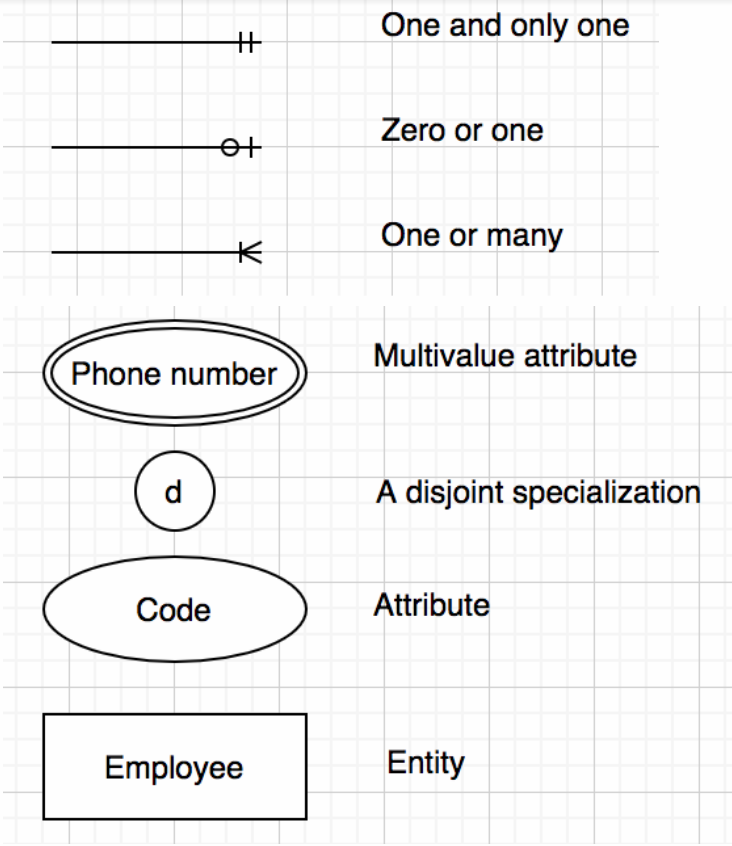
\includegraphics[width=0.5\textwidth]{Photos/Notation.png}}
    \end{figure}
\end{itemize}
\newpage

%% End of description %%
Below is the drawing of \textbf{Enhanced Entity-Relationship Diagram}:
\begin{figure}[!ht]
    \centering
    \fbox{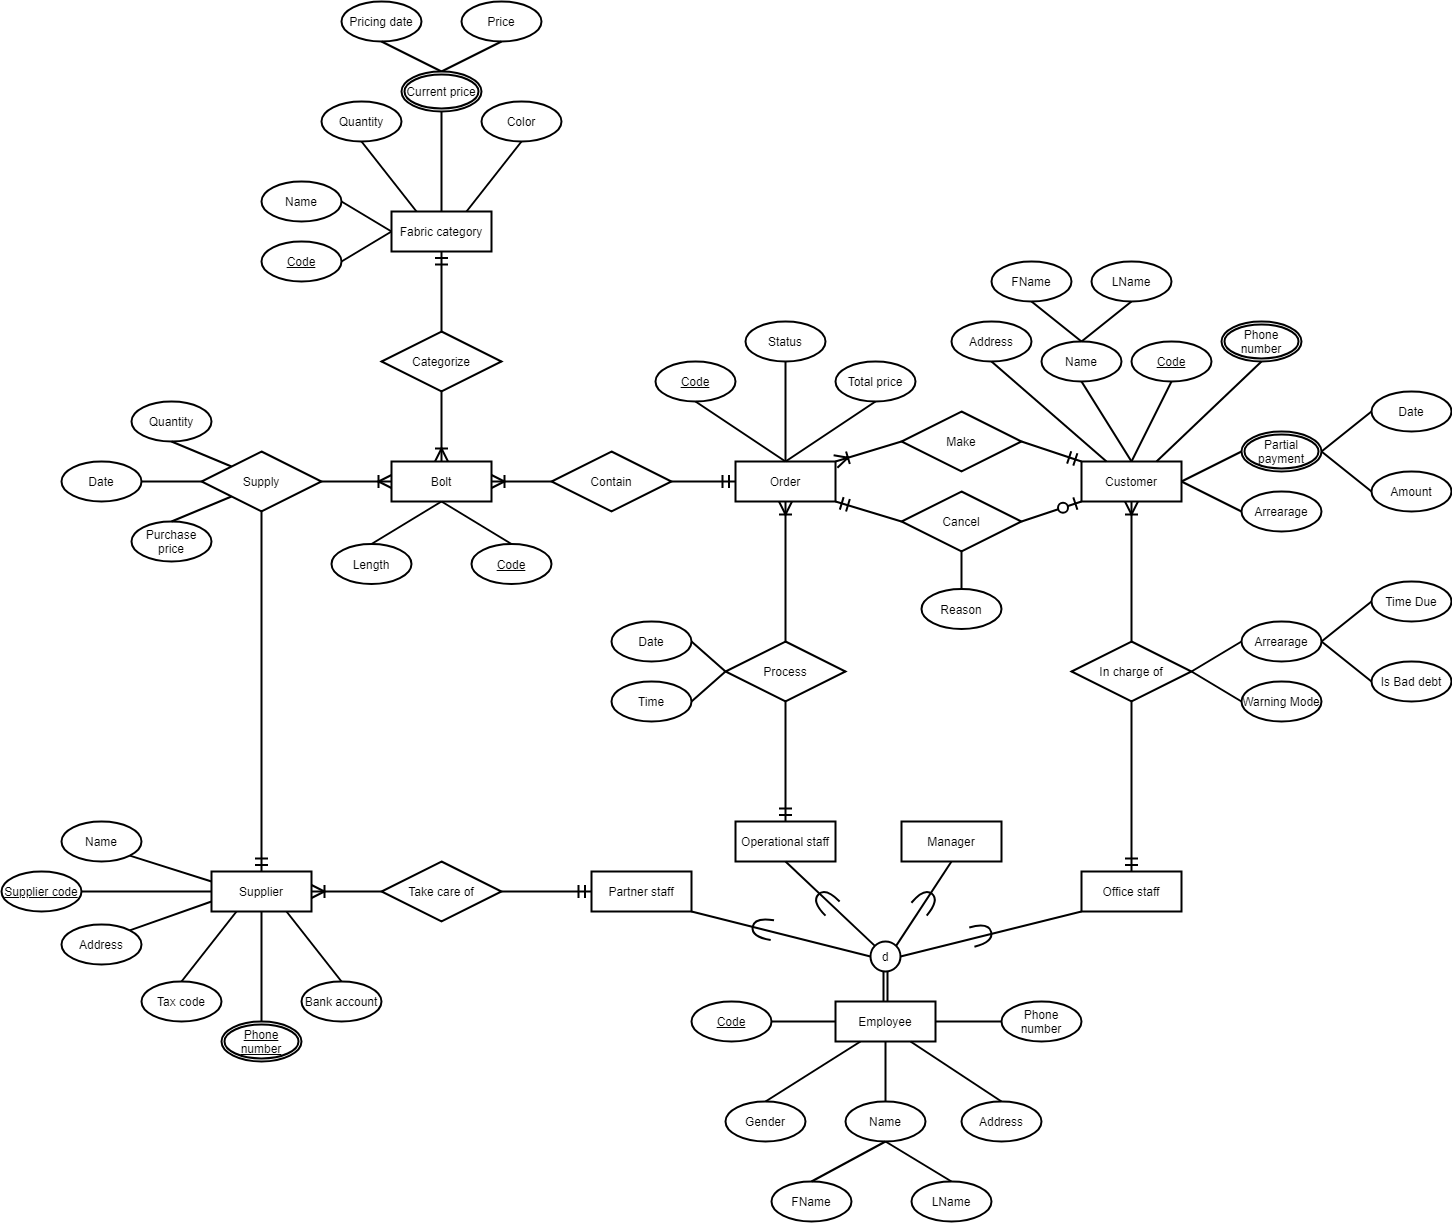
\includegraphics[width=0.9\textwidth]{Photos/EERD.png}}
\end{figure}

\newpage
%%%%%%%%%%%%%%%%%%%%%%%%%%%%%%%%%
\section{Mapping EERD to Relational Databases Schema}
For the mapping to relation databases schema, here is our brief description :
%% Description goes here %%
\begin{itemize}
    \item Relation "FabricCategory" has a unique "FabricCode" attribute, it will keep track of name, quantity in stock, date, quantity, and color of the specific category.
    \item Relation "CurrentFabricPrice" keeps track of the current price for each category as a fabric category has many current price at many time points.
    \item Relation "Bolt" has a unique code, with its length, supplier info, quantity, price and is linked to a category through "CategoryCode".
    \item Relation "Supplier" has a unique "SupplierCode", name, address, bank account of a supplier, and tax code.
    \item Relation "Employee" has a unique code, first name, last name, address, phone number, gender and the type of their job (Manager, Partner staff, Operational staff, and Office staff).
    \item Relation "Customer" has a unique code, first name, last name, address, the code of the employee who is currently in charge of, a flag indicates the "warning" mode by the system to alert the agency, the current arrearage and the time it has exist until now, and a flag to see if he/she is in a bad debt (has been in warning mode for more than 6 months). 
    \item Relation "PartialPayment" records the date and time when a customer makes a partial payment along with his/her unique code.
    \item Relation "SupplierPhoneNumber" and relation "CustomerPhoneNumber" records phone number(s) of a supplier and phone number(s) of a customer, respectively.
    \item Relation "Order" has its unique code, 2 foreign keys are the code of the customer who owns this order and the code of the Employee who processes this order, a total price of the order, process date and time, status of the order (including: "new", "ordered", "partial paid", "full paid" and "cancelled"), a flag to indicate if the order has been cancelled, and the reason for the cancellation (show NULL value if there is no cancellation).
\end{itemize}
%% End of description %%

Below is the drawing of EERD Mapping to {Relational databases schema}: 
\begin{figure}[!ht]
    \centering
    \fbox{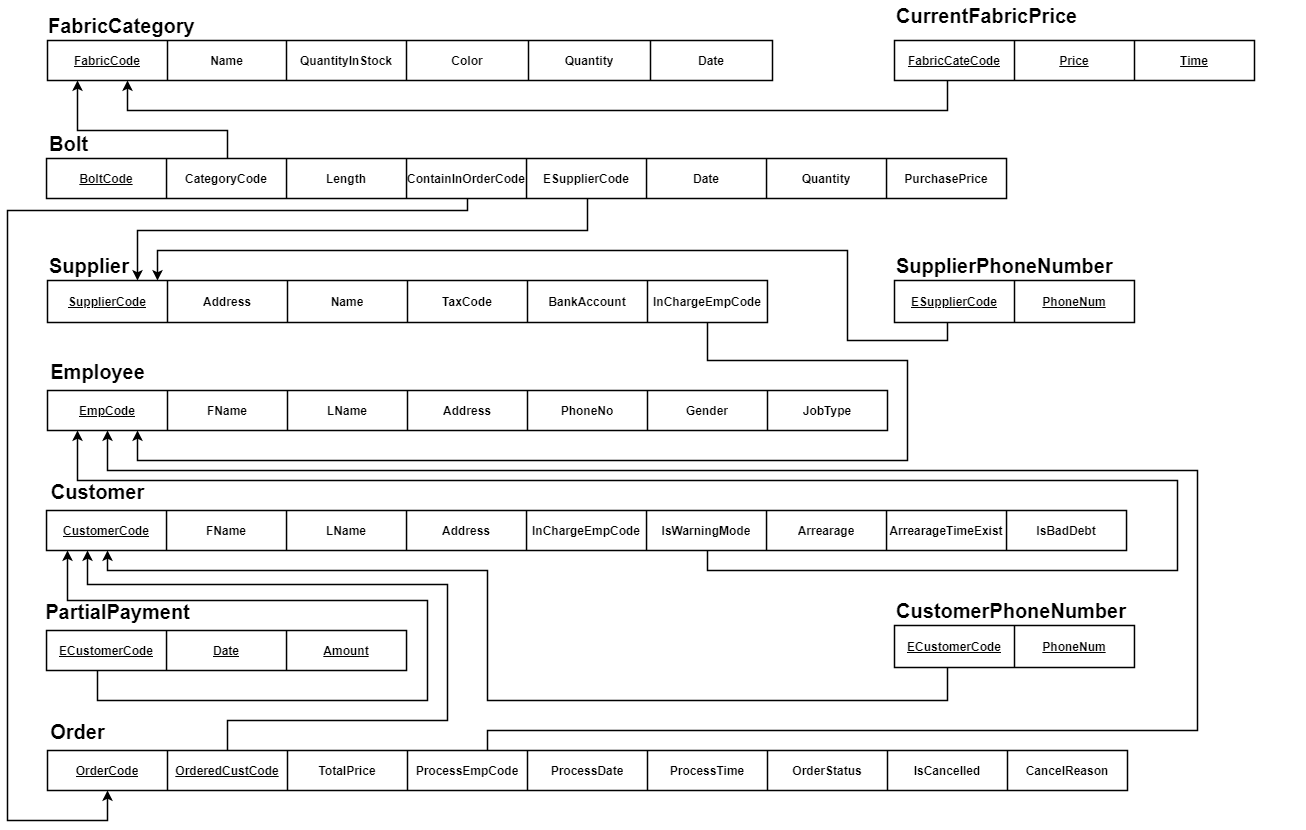
\includegraphics[width=0.95\textwidth]{Photos/Schema.png}}
\end{figure}

\newpage
%%%%%%%%%%%%%%%%%%%%%%%%%%%%%%%%%
\section{Constraints Identification}
Here are some constraints that we additionally identified due to the limit of (Enhanced) Entity-Relationship Diagram. That is, they appeared in the specification of the problem, but it is not possible to display them all on the diagram.
\begin{itemize}
    \item A bolt’s specific category such as : silk, khaki, crewel, jacquard, faux silk, and damask might not be displayed properly. A category code will be the primary key to determine instead.
    \item Order status can’t be determined from the EER Diagram, including “new”, “ordered”, “partial paid”, “full paid”. However, “IsCancelled” status with a Boolean data type (It is easier to get from the relation schema), along with its reason can be displayed, and only be in use if the “IsCancelled” value is TRUE. This situation only occurs when the customer cancel the order.
    \item Whenever the customer makes a new partial payment, the value of arrearage decreases. In the other hand, whenever the customer buys a bolt without paying completely the amount, the value of the arrearage will be increased.
    \item If the value of the “OrderStatus” attribute of the “Order” entity is “Cancelled” or the value "IsCancelled" is TRUE, the value of the “Reason” attribute of the “Cancel” relationship must not be NULL. 
    \item If the “Arrearage” attribute of the “In charge of” relationship is over \$2000, the “Warning mode” attribute of that relationship must be changed to TRUE. If “Warning mode” stays TRUE for 6 months, the arrearage is marked as “bad debt”. 
    \item “Manager” entity, a subclass of “Employee” superclass, currently has no use or any relationship yet, but still exists in the EER Diagram to fulfill the specification.
    \item It is not sure which the staff is in charge of tracking the history payment for the customer, so we chose the office staff for our work.

\end{itemize}


%%%%%%%%%%%%%%%%%%%%%%%%%%%%%%%%%

\end{document}

